\addchap{Die Fakultät Informatik}

Der \emph{Andreas-Pfitzmann-Bau} (kurz APB, häufig auch einfach \glqq{}Fak\grqq{} oder INF genannt), das Gebäude welches die Fakultät Informatik beherbergt, wird in den nächsten 3 bis 5 Jahren euer zweites Zuhause werden.
Viele Lehrveranstaltungen und Übungen werden hier stattfinden. Mit zunehmender Semesterzahl werdet ihr immer weniger über den Campus gescheucht und immer mehr Veranstaltungen werden hier stattfinden.
Doch was hat dieser Bau eigentlich zu bieten außer einer Menge grüner Farbe und der Skulptur im Foyer?

\begin{figure}[h!]
\centering
\includegraphics[width=\linewidth]{img/panorama_fakultaet.jpg}
\caption*{\small \textit{Der Andreas-Pfitzmann-Bau von vorne - Foto: Lucas Vogel}}
\end{figure}

Der wesentliche Unterschied zwischen diesem Gebäude und den anderen auf dem Campus ist, dass es rund um die Uhr geöffnet ist. Auch wenn nachts mal die Türen verschlossen sein sollten, wird euch der Nachtwächter gerne gegen Vorlage eures Studentenausweises die Tür öffnen und auf Wunsch auch einen der Seminarräume im Erdgeschoss aufschließen. 
Auf die PC-Pools müsst ihr nachts zwar verzichten, einer nächtlichen Lernorgie sollte aber trotzdem nichts im Wege stehen.

\begin{figure}[h!]
\centering
\includegraphics[width=\linewidth]{img/panorama_teich.jpg}
\caption*{\small \textit{Der Andreas-Pfitzmann-Bau hinten raus - Foto: Lucas Vogel}}
\end{figure}

Außerdem können wir einen ziemlich schicken Außenbereich unser Eigen nennen. Mit Teich, viel Platz auf der Wiese zum Rumlümmeln und Außensteckdosen, die den Energiebedarf eines Informatikers voll Schaffenskraft mühelos stillen können.

Eine Menge Sitzgelegenheiten auf den Gängen aller Etagen bieten euch auch in der Prüfungsphase genügend Platz, um euch mit euren Lerngruppen auf die anstehenden Prüfungen vorzubereiten. Das \emph{ascii} wird dabei gerne euren Koffeinbedarf stillen.

% TODO: Change this to minisec? Adjust formatting for more :sparkle:? Same for Games Night!
\minisec{ascii - Das Café in der Fakultät}

Bereits seit 2007 existiert im Gebäude der Fakultät Informatik das ascii, ein Café betrieben von Studenten für Studenten, Mitarbeiter und Besucher, kurzum: für jeden.
Das ascii hat alles was ein richtiges Café so braucht: Kaffee, Kuchen, Bagels so wie alles was Nerds an der Fakultät so brauchen: Koffeinhaltige Kaltgetränke!
Zudem zählt das ascii zu den wenigen Adressen auf dem Campus, in denen man neben Club Mate auch Kolle Mate und Premium Cola erhält.
Hinter dem Tresen stehen Studenten, die gerne an einem Tag in der Woche noch ein paar Stündchen ihrer Freizeit zur Verfügung stellen.

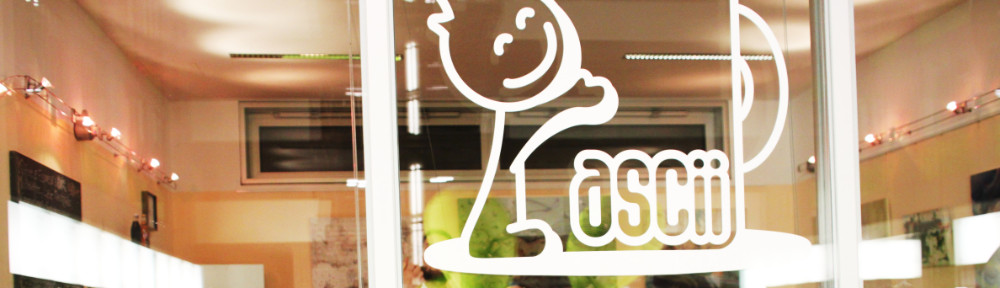
\includegraphics[width=\linewidth]{img/ascii.jpg}

Das ascii wird von einem studentischen Verein betrieben und ist seit seiner Gründung eine zentralen Anlaufstelle für jede und jeden an der Fakultät.
Hier treffen sich Studenten, Mitarbeiter und Professoren um ihre Pausen zu verbringen,
zu arbeiten oder einfach ihren Koffeinhaushalt aufzufüllen.
Auf den gemütlichen Sofas kann man die Zeit wunderbar an sich vorbei streichen lassen,
gemeinsam an Projekten arbeiten, lernen, programmieren oder einfach nur mit seinen Kommilitonen plaudern.
Du kennst noch niemanden an der Fakultät?
Du hast Fragen oder Gesprächsbedarf?
Wenn du ins ascii kommst, wirst du schnell sehen, dass an dem Vorurteil, Nerds seien nicht sozial, absolut nichts dran ist.

Wenn du jetzt Lust bekommen hast, das ascii zu besuchen oder sogar als Mitglied selbst mitzumachen, dann komm doch einfach mal vorbei und sag Hallo!

Weitere Hinweise findest du auf \link{https://www.ascii-dresden.de/}.

\textit{Wir öffnen in der Vorlesungszeit Montag bis Donnerstag von 9 bis 17 Uhr und Freitags von 9 bis 15 Uhr. Dazwischen sind wir aber auch häufig im Café anzutreffen.}

\minisec{Studentenklub Count Down}

\begin{wrapfigure}{l}{3.25cm}%
  \vspace{-.5cm}
  
\includegraphics[width=\linewidth]{img/countdown}
  \vspace{-1cm}
\end{wrapfigure}

Um einen Ort für gemeinsame Treffen und Aktivitäten zu haben, betreibt der Studentenklub IZ e.V. das Count Down.
Dieses befindet sich im Keller des Wohnheims Güntzstraße 22 Eingang C und liegt damit auf halbem Weg zwischen Campus und Neustadt.
Mit einer Mischung aus gemütlichen Kneipenabenden und verschiedenen Partys begleitet es dein Studentenleben, selbstverständlich zu studentischen Preisen!

Montags findet ein traditioneller und fast schon nostalgischer Spieleabend statt.
Damit es nicht langweilig wird, hat das Count Down eine große Auswahl an verschiedenen Brett- und Kartenspielen parat.

Bei den Erasmus-Partys hast du jeden Dienstag die Gelegenheit, gemeinsam mit ausländischen Studenten zu feiern und deren Kulturen kennen zu lernen.

\begin{wrapfigure}{r}{6.9cm}%
  \vspace{-.4cm}
  \hspace{.03\linewidth}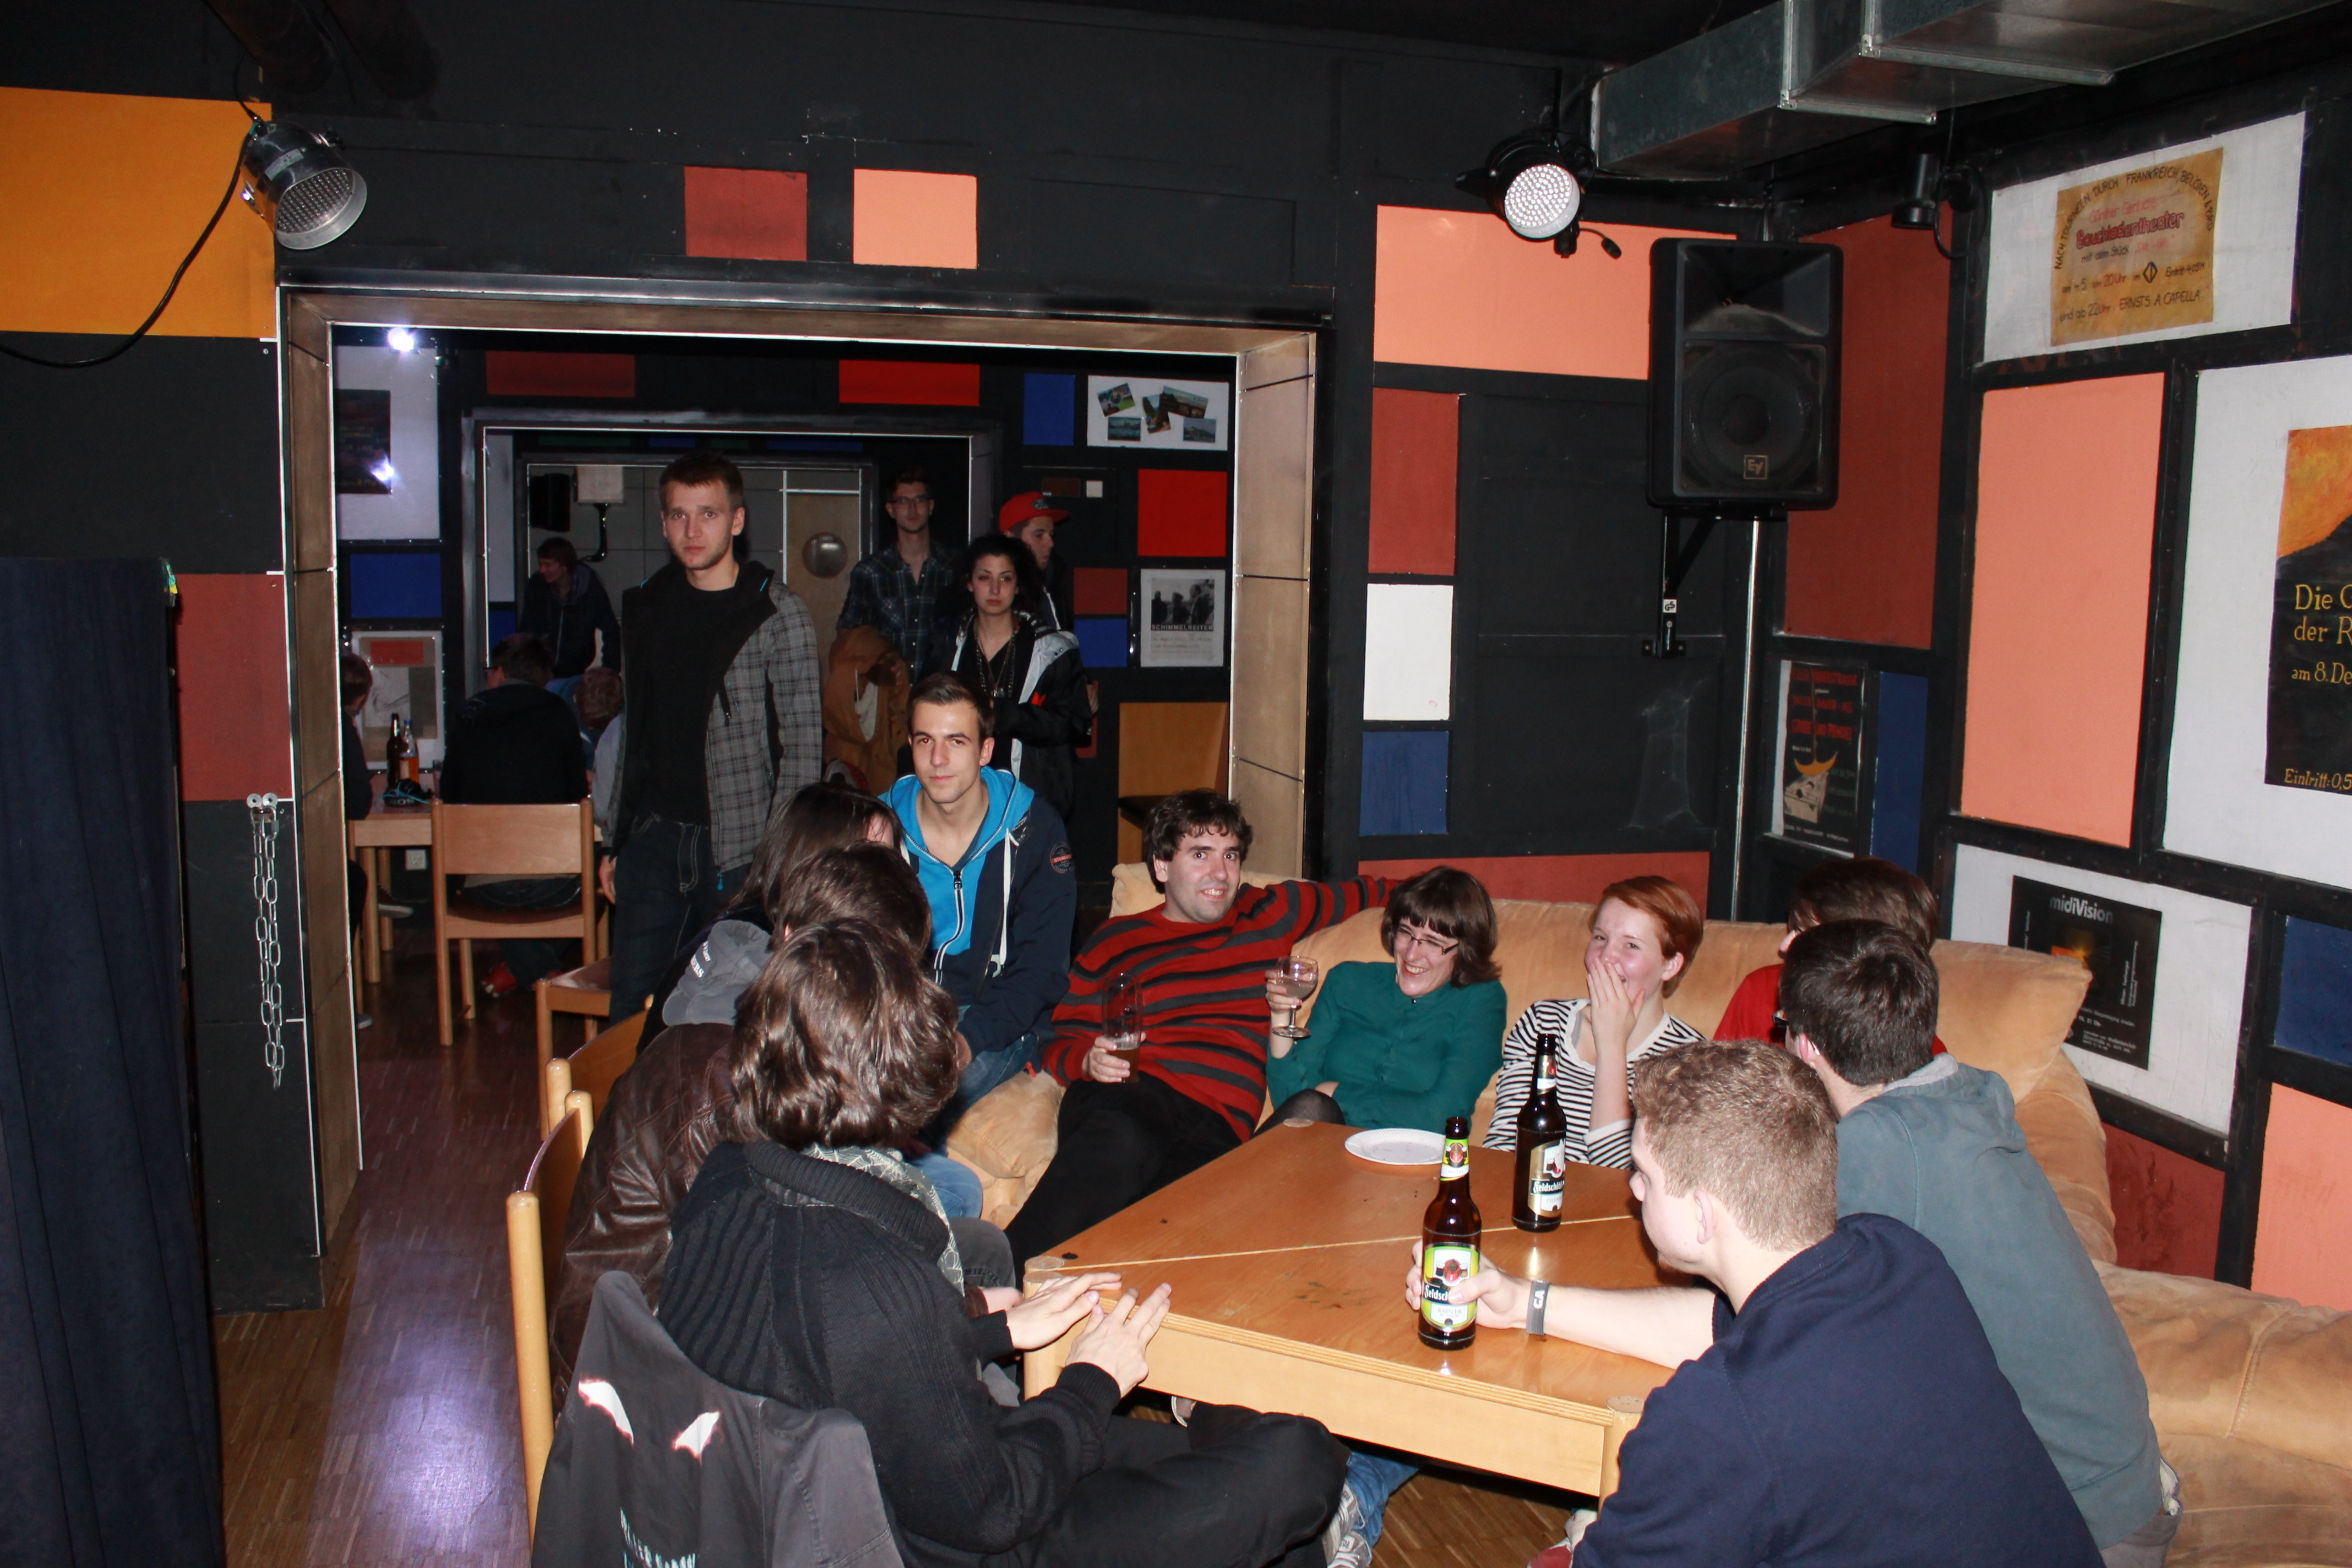
\includegraphics[width=.96\linewidth]{img/ese2013/cd.jpg}
  \vspace{-.4cm}
\end{wrapfigure}

Darüber hinaus gibt es auch viele Veranstaltungen, die nicht im festgeschriebenen Rhythmus stehen, aber trotzdem immer wieder stattfinden.
Dazu gehören unter anderem ein Skatturnier, Cocktail- und Werewolfabende in englischer Sprache, sowie der Metalalterabend.
Den aktuellen Plan findest du unter \link{https://countdown-dresden.de} und auf dem Flyer, den du in der ESE-Tüte gefunden hast ;-)

Du willst gern einmal selbst auf der Bühne stehen?
Ob mit der Blockflöte oder einem spannenden Reisebericht:
Auch dafür ist Platz im Klub und Kalender!

Und solltest du keine fremden Zuschauer haben wollen, sondern einfach mit deinen Freunden eine Party außerhalb deiner eigenen vier Wände geben, bist du ebenfalls beim Count Down genau richtig.
An allen Tagen, an denen keine Veranstaltung geplant ist (insbesondere am Freitag und Samstag), hast du die Möglichkeit, den Klub zu studentisch günstigen Preisen zu mieten, Barpersonal, Aufräumen und Putzen inklusive.
Schau einfach auf die Homepage und reservier' einen Termin!

Das reicht dir immer noch nicht?
Du möchtest das Studentenklubleben gern selbst mit gestalten?
Du triffst gerne viele neue, nette Leute?
Du hast vielleicht sogar weitere Ideen für interessante Veranstaltungen?
Du möchtest gern einmal selbst an der Bar stehen und dabei nicht den Chef im Nacken sitzen, sondern den Spaß im Vordergrund stehen haben?
Sprich die Mitglieder einfach direkt an, neue Mitglieder sind immer herzlich willkommen.

Ob als Gast oder als neues Mitglied - das Count Down freut sich, dich bald im Klub begrüßen zu dürfen.

\minisec{Spieleabende}

Etwa einmal im Monat wird in der Fakultät vom FSR ein Spieleabend ausgerichtet. Start ist dabei immer um 18:30 Uhr im Foyer. Dabei stellt der FSR sein umfangreiches Angebot an analogen Spielen zur Verfügung, sodass eine ganze Menge an Spielen schon von Haus aus da sind. Wollt ihr etwas spielen, was nicht da ist, bringt es am besten mit! Oft sind auch schnell Leute gefunden, die mal ein neues Spiel ausprobieren wollen.

Hin und wieder finden sich auch ein paar Leute, die an dem Abend ihre Notebooks mitbringen und eine kleine LAN-Party schmeißen oder ihre Spielekonsole mitbringen, um über einen der Beamer der Seminarräume mit anderen zusammen zu spielen.

Für Knabbereien und Getränke wird gesorgt, das \emph{ascii} hat in der Regel zu Spieleabenden geöffnet. Wenn das Wetter mitspielt, ist auch das \emph{Count Down}, ein Dresdner Studentenclub, zur Stelle und verkauft Heißes vom Grill sowie alkoholische Getränke.

Es lohnt sich also auf jeden Fall, vorbei zu schauen und bei einer Mate und einer frischen Bratwurst neue Leute kennenzulernen!

\pagebreak

\
\thispagestyle{empty}
\AddToShipoutPicture*{\put(0,0){%
\parbox[b][\paperheight]{\paperwidth}{%
\vfill
\centering
\refstepcounter{dummy}
\label{spieleabendplakat}
\includegraphics[width=\dimen107,height=\dimen108,keepaspectratio]{img/spieleabend.png}%
\vfill
}}}
